% ============================================================
% config.tex
% Packages, layout, colors, custom commands, glossary, acronyms
% ============================================================

% ---------- Page geometry (ESPRIT guide: 2.5 cm margins) ----------
\usepackage[a4paper,margin=2.5cm]{geometry}

% ---------- Language ----------
\usepackage[french,english]{babel}
\selectlanguage{english}

% ---------- Fonts / encoding ----------
\usepackage[utf8]{inputenc}
\usepackage[T1]{fontenc}
\usepackage{lmodern}
\usepackage{times}          % Times New Roman-like body font (guide requirement)
\usepackage{microtype}
\setlength{\emergencystretch}{3em} % reduces overfull lines from long inline \texttt{} paths

% ---------- Line spacing / paragraphs (guide: 1.15, first-line indent 0.5 cm) ----------
\usepackage{setspace}
\setstretch{1.15}
\setlength{\parindent}{0.5cm}
% every paragraph starts with an indent, also the first one after a heading
\usepackage{indentfirst}

% ---------- Color ----------
\usepackage[table]{xcolor}
\definecolor{espritred}{RGB}{200,30,45}
\definecolor{espritdarkred}{RGB}{130,20,35}
\definecolor{espritgraydark}{RGB}{90,90,90}
\definecolor{espritgraylight}{RGB}{180,180,180}
\definecolor{codebg}{RGB}{245,245,245}
\definecolor{codekw}{RGB}{0,90,150}
\definecolor{codecomment}{RGB}{110,110,110}
\definecolor{codestring}{RGB}{150,30,30}

% ---------- Graphics / figures ----------
\usepackage{graphicx}
\graphicspath{{images/}{images/graphs/}{images/screenshots/}{images/logos/}{diagrams/}}
\usepackage{float}
\usepackage{subcaption}

% ---------- Page breaks ----------
% Figures and tables float ([htbp]) so that the text keeps filling a page instead of
% leaving an empty band when a figure does not fit; these limits let large figures
% share a page with text.
\renewcommand{\topfraction}{0.9}
\renewcommand{\bottomfraction}{0.8}
\renewcommand{\textfraction}{0.07}
\renewcommand{\floatpagefraction}{0.8}
\setcounter{topnumber}{3}
\setcounter{bottomnumber}{2}
\setcounter{totalnumber}{4}
% Pages that hold only figures or tables start at the top instead of being centred.
\makeatletter
\setlength{\@fptop}{0pt}
\setlength{\@fpsep}{\floatsep}
\setlength{\@fpbot}{0pt plus 1fil}
\makeatother
% A heading is never left at the bottom of a page with only a line or two under it:
% \Needspace{h} starts a new page when less than h of the page is left (same logic as
% the needspace package, defined here because that package is not installed).
\usepackage{etoolbox}
\makeatletter
\newcommand{\Needspace}[1]{\par\penalty-100\begingroup
  \setlength{\dimen@}{#1}%
  % On a page that has no text yet, the room left is \vsize, which LaTeX has already
  % reduced by the figures and tables placed at the top of that page.
  \ifdim\pagegoal=\maxdimen \dimen@ii\vsize \else \dimen@ii\pagegoal \fi
  \advance\dimen@ii-\pagetotal
  \ifdim\dimen@>\dimen@ii
    \ifdim\pagegoal=\maxdimen \ifdim\vsize<\textheight \null\fi\fi
    \ifdim\dimen@ii>\z@ \vfil\fi
    \break
  \fi\endgroup}
\makeatother
\pretocmd{\section}{\Needspace{13\baselineskip}}{}{\PackageWarning{config}{PATCHFAIL section}}
\pretocmd{\subsection}{\Needspace{7\baselineskip}}{}{\PackageWarning{config}{PATCHFAIL subsection}}
\pretocmd{\subsubsection}{\Needspace{6\baselineskip}}{}{\PackageWarning{config}{PATCHFAIL subsubsection}}
% Loaded after the heading check so that pending figures are placed first. A figure
% stays near its section: it may share a page with the start of the next one.
\usepackage[section,above,below]{placeins}
% When a section starts while figures of the previous one are still waiting, placeins
% ejects the page and, if they do not all fit at the top of the next one, uses \clearpage,
% which leaves a page with one figure and the new section alone on the page after. Here
% the waiting figures are placed page by page instead, and the text goes on under the
% last of them.
\makeatletter
\def\FloatBarrier{\par\begingroup\let\@elt\relax\@tempcnta\z@
  \loop
    \edef\@tempa{\@deferlist\@dbldeferlist}%
    \ifx\@tempa\@empty \@tempswafalse \else \@tempswatrue \fi
    \if@tempswa
      \ifdim\pagegoal=\maxdimen \ifx\@toplist\@empty \@tempcnta9 \fi\fi
      \ifnum\@tempcnta>6 \clearpage \@tempswafalse \fi
    \fi
  \if@tempswa
    \advance\@tempcnta\@ne
    \ifdim\pagegoal=\maxdimen \null\fi
    \newpage
  \repeat
  \endgroup\@fb@topbarrier}
\makeatother
\clubpenalty=10000
\widowpenalty=10000

% ---------- Tables ----------
\usepackage{amsmath}
\usepackage{booktabs}
\usepackage{longtable}
\usepackage{multirow}
\usepackage{array}
\usepackage{tabularx}
% prose columns of tables: ragged right, no stretched spaces
\newcolumntype{P}[1]{>{\raggedright\arraybackslash}p{#1}}
\newcolumntype{Y}{>{\raggedright\arraybackslash}X}
% long tables are not floats: they start right under the text that introduces them and
% continue on the next page with their header repeated
\usepackage{xltabular}
\setlength{\LTcapwidth}{\textwidth}
\setlength{\LTpre}{\medskipamount}
\setlength{\LTpost}{\medskipamount}

% ---------- Diagrams ----------
\usepackage{ifthen}
\usepackage{tikz}
\usetikzlibrary{arrows.meta,positioning,shapes.geometric,shapes.multipart,fit,backgrounds,calc,shadows}
\usepackage{pgfgantt}
\usepackage{pgfplots}
\pgfplotsset{compat=1.18}

% ---------- Code listings ----------
\usepackage{listings}
\lstdefinestyle{codestyle}{
    backgroundcolor=\color{codebg},
    commentstyle=\color{codecomment}\itshape,
    keywordstyle=\color{codekw}\bfseries,
    stringstyle=\color{codestring},
    basicstyle=\ttfamily\footnotesize,
    breakatwhitespace=false,
    breaklines=true,
    captionpos=b,
    keepspaces=true,
    numbers=left,
    numbersep=6pt,
    numberstyle=\tiny\color{gray},
    showspaces=false,
    showstringspaces=false,
    showtabs=false,
    tabsize=2,
    frame=single,
    framerule=0.3pt,
    rulecolor=\color{gray!40}
}
\lstset{style=codestyle}

% ---------- Hyperlinks / PDF bookmarks ----------
\usepackage{hyperref}
\hypersetup{
    colorlinks=true,
    linkcolor=blue,
    citecolor=blue,
    urlcolor=blue,
    filecolor=blue,
    bookmarksnumbered=true,
    bookmarksopen=true,
    plainpages=false,
    pdfpagelabels=true,
    pdftitle={CANvisionNative - PFE Report},
    pdfauthor={Mohamed Mootaz Ben Kraiem},
    pdfsubject={Final Year Engineering Project Report},
}
\usepackage[nameinlink,noabbrev]{cleveref} % must load after hyperref

% ---------- Acronyms / Glossary ----------
\usepackage[acronym,nomain,nonumberlist]{glossaries}
\makeglossaries
% ============================================================
% acronyms.tex — List of abbreviations used in the report
% ============================================================

\newacronym{can}{CAN}{Controller Area Network}
\newacronym{canfd}{CAN FD}{CAN with Flexible Data-rate}
\newacronym{uds}{UDS}{Unified Diagnostic Services}
\newacronym{isotp}{ISO-TP}{ISO Transport Protocol (ISO 15765-2)}
\newacronym{obd}{OBD-II}{On-Board Diagnostics, second generation}
\newacronym{bms}{BMS}{Battery Management System}
\newacronym{ids}{IDS}{Intrusion Detection System}
\newacronym{ml}{ML}{Machine Learning}
\newacronym{ai}{AI}{Artificial Intelligence}
\newacronym{llm}{LLM}{Large Language Model}
\newacronym{nvd}{NVD}{National Vulnerability Database}
\newacronym{rag}{RAG}{Retrieval-Augmented Generation}
\newacronym{iforest}{IF}{Isolation Forest}
\newacronym{kmeans}{K-Means}{K-Means Clustering}
\newacronym{svm}{SVM}{Support Vector Machine}
\newacronym{lof}{LOF}{Local Outlier Factor}
\newacronym{dbc}{DBC}{CAN Database}
\newacronym{ev}{EV}{Electric Vehicle}
\newacronym{mf4}{MF4}{ASAM Measurement Data Format version 4}
\newacronym{api}{API}{Application Programming Interface}
\newacronym{rest}{REST}{Representational State Transfer}
\newacronym{gui}{GUI}{Graphical User Interface}
\newacronym{wpf}{WPF}{Windows Presentation Foundation}
\newacronym{mvvm}{MVVM}{Model-View-ViewModel}
\newacronym{json}{JSON}{JavaScript Object Notation}
\newacronym{http}{HTTP}{Hypertext Transfer Protocol}
\newacronym{csv}{CSV}{Comma-Separated Values}
\newacronym{ecu}{ECU}{Electronic Control Unit}
\newacronym{dos}{DoS}{Denial of Service}
\newacronym{fp}{FP}{False Positive}
\newacronym{fn}{FN}{False Negative}
\newacronym{fps}{FPS}{Frames Per Second}
\newacronym{pfe}{PFE}{Projet de Fin d'Études (Final Year Engineering Project)}
\newacronym{sdk}{SDK}{Software Development Kit}
\newacronym{qa}{QA}{Quality Assurance}
\newacronym{rc}{RC}{Release Candidate}
\newacronym{up}{UP}{Unified Process}
\newacronym{ttup}{2TUP}{Two Track Unified Process}
\newacronym{uml}{UML}{Unified Modeling Language}
\newacronym{furps}{FURPS+}{Functionality, Usability, Reliability, Performance, Supportability, plus constraints}


% ---------- Bibliography (IEEE style) ----------
\usepackage[backend=biber,style=ieee,sorting=none]{biblatex}
\addbibresource{references.bib}
\setlength{\bibitemsep}{3pt}

% ---------- Headers / footers ----------
\usepackage{fancyhdr}
\setlength{\headheight}{14pt}
\pagestyle{fancy}
\fancyhf{}
\fancyhead[L]{\small\leftmark}
\fancyhead[R]{\small\thepage}
\renewcommand{\headrulewidth}{0.4pt}
% ESPRIT band of triangles along the bottom edge of the page. The cover, the dedication and
% the back cover use the empty style, so they are the only pages without it.
\newcommand{\espritband}{\begin{tikzpicture}[remember picture,overlay]
  \node[anchor=south west,inner sep=0pt] at (current page.south west)
    {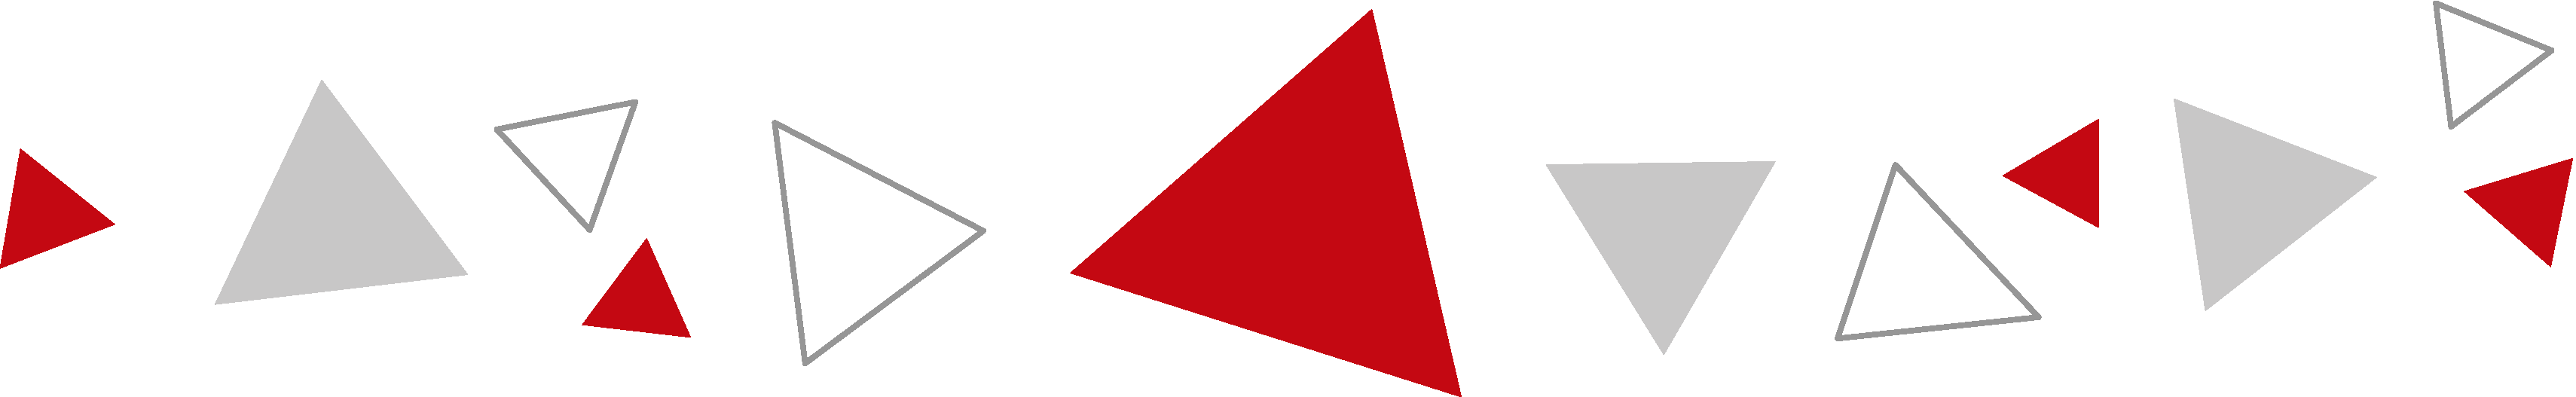
\includegraphics[width=\paperwidth,height=40pt]{esprit_band.pdf}};
\end{tikzpicture}}
\fancyfoot[C]{\espritband}
\fancypagestyle{plain}{\fancyhf{}\fancyfoot[C]{\espritband\raisebox{14pt}[0pt][0pt]{\thepage}}\renewcommand{\headrulewidth}{0pt}}

% ---------- Section title numbering depth ----------
\setcounter{secnumdepth}{3}
% Sections are numbered within their chapter without the chapter number (1, 1.1, 1.1.1),
% so that no heading has more than three levels of numbering. Figures and tables keep the
% chapter number (Figure 2.1).
\renewcommand{\thesection}{\arabic{section}}
% A reference to a section remembers its chapter: \Sref{label} prints "Section 3" inside the
% same chapter and "Section 3 of Chapter 4" from another chapter.
\makeatletter
\DeclareRobustCommand{\chmark}[1]{\gdef\lastrefch{#1}}
\gdef\lastrefch{}
\renewcommand*{\p@section}{\chmark{\thechapter}}
\renewcommand*{\p@subsection}{\chmark{\thechapter}}
\renewcommand*{\p@subsubsection}{\chmark{\thechapter}}
\newcommand*{\thischapterid}{\thechapter}
\newcommand*{\Sref}[1]{%
  \gdef\lastrefch{}\sbox\z@{\ref*{#1}}%
  Section~\ref{#1}%
  \begingroup\edef\@tempa{\lastrefch}\edef\@tempb{\thischapterid}%
  \ifx\@tempa\@empty\else\ifx\@tempa\@tempb\else\ of Chapter~\lastrefch\fi\fi\endgroup}
\makeatother
\setcounter{tocdepth}{3}

% ---------- Custom commands ----------
\newcommand{\todofill}[1]{\textbf{[TO FILL: #1]}}
\newcommand{\code}[1]{\texttt{#1}}
% a logo with its name under it; the optional argument sets the height of the logo
\newcommand{\techlogo}[3][1.1cm]{\begin{tabular}[b]{@{}c@{}}\rule[-0.55cm]{0pt}{1.1cm}\raisebox{-0.5\height}{\includegraphics[height=#1]{#2}}\\[2pt]\footnotesize #3\end{tabular}}
